\chapter{Funding Ideas: Demonstration Before Capital}

This chapter follows a short School of Hard Knocks exchange, curated by LazyingArt LLC through Video2Book, about how an entrepreneur should approach funding when the starting point is only an idea. There is no blackboard mathematics in the source material. The useful structure is instead a compact commercial logic: capital is easier to ask for when the founder can show evidence, and the strongest evidence is not advertising polish but a product that real users accept.

\section{The Funding Question}

The opening question is plain: what should people do if they are trying to get funding for their ideas in order to build companies? We should keep the question in that practical form. The point is not yet venture finance, term sheets, or valuation. It is the earlier problem of evidential strength.

Let \(I\) denote an idea-only proposal and let \(D\) denote a demonstrable artifact: a sample, prototype, mockup, or any other object that can be shown and reacted to. The speaker's first move is to distinguish these two cases:
\begin{equation}
I \;\prec_{\mathrm{funding\ evidence}}\; I + D .
\end{equation}
This is not a formula quoted from the interview. It is a compact notation for the interview's practical claim: something demonstrable is stronger than an idea alone.

\subsection{Question \& Answer}

\paragraph{Question.}
Can a founder get funding for an idea before the company has anything real to show?

\paragraph{Answer.}
The speaker's answer is cautious and direct. It always helps to have something demonstrable and not just an idea. Ideas are difficult to get funded because they leave too much for the investor to imagine, infer, or trust. A sample, or some other concrete demonstration, goes a long way because it changes the conversation from belief to evidence.

\section{Ideas Are Hard To Fund}

An idea has direction, but it has very little observed behavior. It can describe a possible company, but it cannot yet show whether the founder can build, whether the product can function, or whether the user will care. In the speaker's terms, ideas are ``really difficult'' to get funded.

We can write the funding case as a strength-of-evidence quantity \(F\), not as a probability and not as a measured dollar amount. The idea-only case starts with a weak evidential base:
\begin{equation}
F(I)=F_{\mathrm{idea}} .
\end{equation}
The difficulty is not that \(F_{\mathrm{idea}}\) is zero. Some founders do raise money on reputation, relationships, or an unusually compelling thesis. But in the ordinary early case described here, the idea by itself does not carry much observable proof.

\begin{remark}
The notation in this chapter is editorial. It gives shape to the business reasoning in the interview, but it should not be read as mathematics written or spoken in the source.
\end{remark}

\section{Making The Idea Demonstrable}

The speaker then gives the practical move: build something that can be demonstrated. The transcript says ``even just a sample'' and then contains a likely garbled phrase, transcribed as ``especially an attack.'' We should not build a special term around that phrase. The safe reading is that the founder should bring some artifact that can be shown.

If \(D\) is the demonstrable object, then the evidential update is:
\begin{equation}
F(I+D)=F(I)+\Delta_D,\qquad \Delta_D>0 .
\end{equation}
The sign of \(\Delta_D\) is the point. The demonstration does not have to be the finished company. It can be a sample. It can be a crude prototype. It can be a concrete enough version of the idea that another person can inspect it, use it, criticize it, or believe that the founder can build further.

\paragraph{Worked evidence update.}
The reasoning can be kept in four steps:
\begin{enumerate}
\item Begin with an idea-only proposal \(I\).
\item The investor sees mainly intention, so the evidence level is \(F(I)\).
\item The founder adds a demonstrable artifact \(D\).
\item The funding case becomes \(F(I+D)=F(I)+\Delta_D\), where the positive increment is the added evidence that the idea can leave the founder's head and become something observable.
\end{enumerate}

This is the first principle of the exchange: before asking capital to move, make the idea visible.

\begin{figure}
\centering
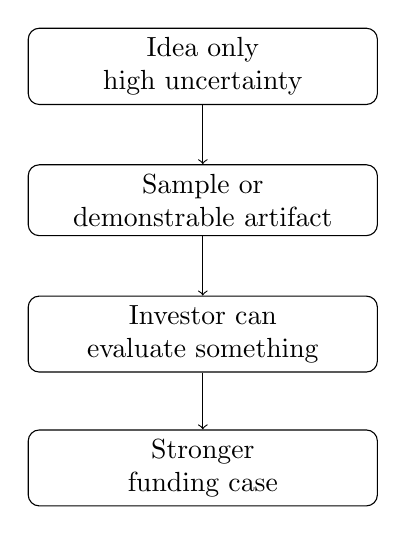
\begin{tikzpicture}[x=1cm,y=1cm]
\node[draw, rounded corners, align=center, text width=4.2cm] (idea) at (0,0) {Idea only\\high uncertainty};
\node[draw, rounded corners, align=center, text width=4.2cm] (demo) at (0,-1.7) {Sample or\\demonstrable artifact};
\node[draw, rounded corners, align=center, text width=4.2cm] (eval) at (0,-3.4) {Investor can\\evaluate something};
\node[draw, rounded corners, align=center, text width=4.2cm] (fund) at (0,-5.1) {Stronger\\funding case};

\draw[->] (idea) -- (demo);
\draw[->] (demo) -- (eval);
\draw[->] (eval) -- (fund);
\end{tikzpicture}
\caption{A transcript-derived evidence ladder. No screenshot is available for this diagram; it is a compact reconstruction of the interview's funding logic.}
\end{figure}

\section{The Dog Food Wars Anecdote}

The speaker then pivots into an old expression, which he places in the 1970s and associates with what he calls, cautiously, the ``dog food wars.'' The details should remain modest: advertising companies were creating many different dog foods, spending money, and putting them on television.

The purpose of the anecdote is not to give a verified business-history case study. It is to make the same evidence principle more vivid. A company may increase attention, but attention is not the same as acceptance. Let \(A\) denote advertising exposure and let \(U\) denote user acceptance. The mistake in the story is to treat exposure as if it implied acceptance:
\begin{equation}
A \uparrow \;\not\Rightarrow\; U \uparrow .
\end{equation}

The product was visible. The product was advertised. But the decisive user in the story was not persuaded by the campaign.

\section{The Market Test}

The turn in the story is simple: the dogs did not like the dog food. The speaker's contrast is sharp because it separates two kinds of evidence. Advertising can prove that a company spent money to get attention. It does not prove that the intended user wants the product.

For a product \(P\), write \(A(P)=1\) when promotion is high and \(U(P)=1\) when the user accepts the product. The dog-food anecdote is the case:
\begin{equation}
A(P)=1,\qquad U(P)=0 .
\end{equation}
From the funding point of view, this is weak evidence, not strong evidence:
\begin{equation}
A(P)=1,\ U(P)=0
\quad\Longrightarrow\quad
F(P)\ \hbox{remains weak as market proof.}
\end{equation}

This is why the anecdote belongs directly after the advice about demonstration. A demonstration is useful only because it can expose reality. If the product fails the user test, the demonstration has still done important work: it has shown that polish and promotion are not enough.

\begin{figure}
\centering
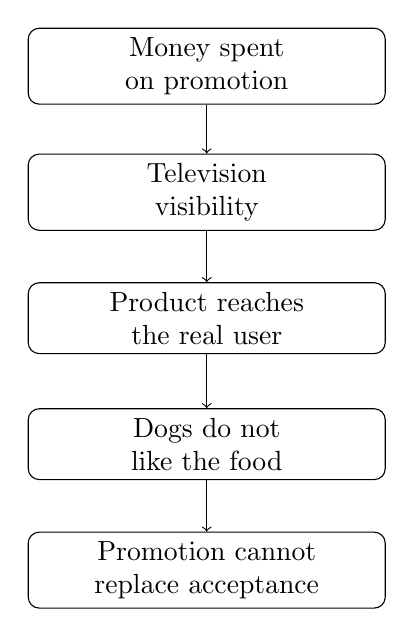
\begin{tikzpicture}[x=1cm,y=1cm]
\node[draw, rounded corners, align=center, text width=4.3cm] (spend) at (0,0) {Money spent\\on promotion};
\node[draw, rounded corners, align=center, text width=4.3cm] (tv) at (0,-1.6) {Television\\visibility};
\node[draw, rounded corners, align=center, text width=4.3cm] (trial) at (0,-3.2) {Product reaches\\the real user};
\node[draw, rounded corners, align=center, text width=4.3cm] (reject) at (0,-4.8) {Dogs do not\\like the food};
\node[draw, rounded corners, align=center, text width=4.3cm] (lesson) at (0,-6.4) {Promotion cannot\\replace acceptance};

\draw[->] (spend) -- (tv);
\draw[->] (tv) -- (trial);
\draw[->] (trial) -- (reject);
\draw[->] (reject) -- (lesson);
\end{tikzpicture}
\caption{The dog-food anecdote as a narrow causal chain: exposure is not the same as validation.}
\end{figure}

\section{Evidence Before Capital}

We can now bring the two halves of the exchange together. The funding question begins with the founder's problem: how do we turn an idea into a fundable company? The answer is not merely to make the idea sound better. It is to reduce uncertainty.

A concise way to write the mechanism is:
\begin{align}
\hbox{idea only} &\longrightarrow \hbox{high investor uncertainty},\\
\hbox{demonstrable artifact} &\longrightarrow \hbox{lower investor uncertainty},\\
\hbox{real user acceptance} &\longrightarrow \hbox{stronger market proof}.
\end{align}
The dog-food story adds the negative version:
\begin{equation}
\hbox{flashy presentation} \not\equiv \hbox{validated demand}.
\end{equation}

The practical lesson is therefore disciplined. If a founder wants funding, the first work is not just persuasion. The first work is to create something that makes persuasion less necessary. A sample, a prototype, or a visible test converts part of the founder's claim into evidence.

\section{Summary}

This short exchange gives one compact rule for early funding: bring evidence, not just an idea. The speaker starts with the founder's question, answers with the value of something demonstrable, and then uses the dog-food anecdote to show why visibility and polish are weaker than product acceptance.

The chapter's reconstructed notation can be summarized in one line:
\begin{equation}
\text{funding strength}
\quad\hbox{comes from}\quad
\text{demonstration}+\text{user evidence},
\quad\hbox{not from idea alone.}
\end{equation}
The careful version is even simpler: before asking investors to believe, give them something real to evaluate.